\documentclass[10pt,twocolumn]{article}
\usepackage[margin=0.68in,columnsep=0.24in]{geometry}
\usepackage[T1]{fontenc}
\usepackage[utf8]{inputenc}
\usepackage{lmodern}
\usepackage{microtype}
\usepackage{amsmath,amssymb,amsthm}
\usepackage{booktabs}
\usepackage{graphicx}
\usepackage{xcolor}
\usepackage{enumitem}
\usepackage{hyperref}

\hypersetup{
  colorlinks=true,
  linkcolor=blue!60!black,
  citecolor=blue!60!black,
  urlcolor=blue!60!black,
  pdftitle={Certified Verification of NEXPTIME-Hardness for Degree-Bounded Local-Sum MPNN Satisfiability},
  pdfauthor={Lluis Eriksson}
}

\newtheorem{proposition}{Proposition}
\newcommand{\QQ}{\mathbb{Q}}
\newcommand{\NN}{\mathbb{N}}
\newcommand{\ZZ}{\mathbb{Z}}
\newcommand{\enc}{\operatorname{enc}}
\newcommand{\push}{\operatorname{push}}
\newcommand{\pop}{\operatorname{pop}}
\newcommand{\relu}{\operatorname{relu}}
\newcommand{\DEGBSAT}{\textsc{DegBSat}}
\newcommand{\NEXP}{\mathsf{NEXP}}
\newcommand{\PSPACE}{\mathsf{PSPACE}}

\title{\vspace{-1.1em}\textbf{Certified Verification of NEXPTIME-Hardness for Degree-Bounded Local-Sum MPNN Satisfiability}}
\author{Lluis Eriksson\thanks{Independent Researcher. Code, Lean~4 proofs, and certificates: MIT License; manuscript and figures: CC-BY-4.0. Prepared with AI coding, formalization, and drafting assistance from Google Antigravity; all proofs, exact-$\QQ$ verifiers, and adversarial tests were independently compiled and verified locally. Repository: \url{https://github.com/lluiseriksson/mpnn-degbsat-nexptime-certificates}}}
\date{November 25, 2026}

\begin{document}
\maketitle
\vspace{-1.4em}

\begin{abstract}
Marco S\"alzer (\texttt{arXiv:2611.32595}, Nov.\ 2026) resolved the exact complexity of degree-bounded satisfiability (\DEGBSAT{}) for local-sum Message Passing Neural Networks (MPNNs) with ReLU activations and rational node labels, closing the gap between $\PSPACE$-hardness and the $\NEXP$ upper bound by proving $\NEXP$-hardness already at fixed degree bound $d = 3$---via a proof architecture proposed by an AI model (GPT-6 Astra). The reduction packs arbitrary-length nondeterministic Turing machine (NTM) tapes into base-$(|\Gamma|+2)$ rational encodings, expresses single-step transitions as a finite union $\Delta$ of rational polyhedra, recognizes $\Delta$ and accepting configurations $\mathcal{F}$ via exact ReLU-FNNs, and verifies $2^{p(|w|)}$-step runs in $p(|w|)+2$ local-sum message-passing layers on degree-$\le 3$ trees. We construct a standalone, zero-dependency \textbf{Lean~4.35.0} formalization of 18 core encoding, polyhedral, ReLU-FNN, and MPNN acceptance theorems (zero \texttt{sorry}, zero warnings, zero \texttt{Classical.choice}) paired with an exact-$\QQ$ four-mode certificate verifier (\texttt{MPNN-DEGBSAT-CERT-1.0}) that executes S\"alzer's full $(h+2)$-layer MPNN $M_w$ without floating-point arithmetic. Across 16 canonical certificates ($0.080$--$114.497\,\mathrm{ms}$, total $286.40\,\mathrm{ms}$), all invariants replay identically over $\QQ$ while rejecting 62/62 live adversarial forgery attacks.
\end{abstract}

\section{Introduction}\label{sec:intro}
Formal verification of Graph Neural Networks asks whether a classifying MPNN accepts any graph violating a safety specification~\cite{barcelo2020logical,saelzer2023fundamental}. For local-sum ReLU MPNNs over arbitrary rational node labels, unbounded-degree satisfiability is undecidable~\cite{benedikt2026decidability}, whereas restricting input graphs to degree at most $d$ (\DEGBSAT{}) restores decidability~\cite{saelzer2023fundamental} with an $\NEXP$ upper bound when $d$ is given in unary~\cite{saelzer2025complexity}. S\"alzer~\cite{saelzer2026degbsat} closed the longstanding $\PSPACE$-vs.-$\NEXP$ gap by proving $\NEXP$-hardness even for fixed degree $d = 3$ (Theorem~6.1 and Corollary~6.2).

The reduction combines four exact rational gadgets:
\begin{enumerate}[leftmargin=*,nosep]
  \item \textbf{Base-$b$ Tape Encoding (Lemma~3.1):} With working alphabet $\Gamma = \{1,\dots,k\}$ and base $b = k + 2$, $\enc(a_1\cdots a_m) = \sum_{i=1}^m a_i b^{-i} + s/((b-1)b^m)$ lies in $I = [1/(b-1), k/(b-1)]$ (width $(k-1)/(k+1) < 1$), $\push_a(x) = (x+a)/b$ and $\pop_a(x) = bx - a$ implement tape shifts, and $\pop_a(\enc(w)) \in I \iff a = \operatorname{head}(w)$.
  \item \textbf{Polyhedral NTM Step Relation (Lemma~4.1):} Single steps and accepting-state padding form a union $\Delta$ of $|\Gamma|(|\delta|+1)$ rational polyhedra in $\QQ^6$, and accepting configurations form $\mathcal{F}$ ($|\Gamma|$ polyhedra in $\QQ^3$), so $T$ accepts $w$ in $\le n$ steps iff $(\enc(c_w), x) \in \Delta^n$ for some $x \in \mathcal{F}$.
  \item \textbf{ReLU-FNN Polyhedral Union Recognizer (Lemma~5.1):} For $S = \bigcup_{i=1}^n \{x : A_i x \le b_i\}$, $N_S(x) = \min_i \sum_j \relu((A_i x - b_i)_j)$ is realized exactly using $\min(x, y) = \relu(x - \relu(x - y))$ and satisfies $N_S(x) \ge 0$ with $N_S(x) = 0 \iff x \in S$.
  \item \textbf{Binary Run-Tree Local-Sum MPNN (Theorem~6.1):} For height $h = p(|w|)$, each node stores $2(h+1)$ typed blocks $(z_t, A_t, B_t)$ of total dimension $d = 14(h+1)$. Layer~$N_1$ evaluates local endpoint-matching, leaf-$\Delta$, and root-$\mathcal{F}$ errors $(x_u^{(1)})_1, (x_u^{(1)})_2 \ge 0$; $h$ sum-aggregation layers propagate non-negative errors to the root $v$; and $N_{h+2}$ outputs $\relu(1 - (x_v^{(h+1)})_1 - (x_v^{(h+1)})_2)$, accepting iff both errors vanish on a degree-$\le 3$ witness of length $2^h$.
\end{enumerate}

\paragraph{Contributions and Scope.}
We do not re-formalize complexity-class many-one reductions or Turing-machine time hierarchies inside Lean~4; instead, we provide an independent machine-checked verification suite for every algebraic, polyhedral, neural, and graph-level invariant of~\cite{saelzer2026degbsat}:
(i)~18 zero-\texttt{sorry}, zero-\texttt{Classical.choice} \textbf{Lean~4.35.0}~\cite{demoura2021lean4} theorems in \texttt{MPNNDegBSat.lean};
(ii)~the zero-floating-point exact-$\QQ$ verifier \texttt{MPNN-DEGBSAT-CERT-1.0};
(iii)~16 canonical certificates (including full exact $(h+2)$-layer $M_w$ execution on degree-$\le 3$ accepting and corrupted graphs); and
(iv)~a 62-attack live adversarial red-team suite with 41-artifact SHA-256 manifest enforcement.

\section{Constructive Lean~4.35.0 Kernel}\label{sec:lean}
The standalone module \texttt{lean/MPNNDegBSat.lean} builds cleanly under Lean~4.35.0 with zero external libraries, zero warnings, and zero \texttt{sorry}. Auditing all 18 theorems via \texttt{\#print axioms} (\texttt{AuditAxioms.lean}) confirms 2 zero-axiom theorems (\texttt{none}), 16 using only \texttt{[propext, Quot.sound]}, and \textbf{0} using \texttt{Classical.choice} or \texttt{Lean.ofReduceBool} (Table~\ref{tab:lean}).

\begin{table}[t]
\centering
\caption{All 18 machine-checked Lean~4.35.0 theorems in \texttt{MPNNDegBSat.lean} (zero \texttt{sorry}, zero \texttt{Classical.choice}).}
\label{tab:lean}
\scriptsize
\setlength{\tabcolsep}{3.0pt}
\begin{tabular}{@{}rlll@{}}
\toprule
\# & Lean Theorem Identifier & Paper Ref. & Axioms \\
\midrule
1 & \texttt{interval\_I\_well\_formed} & Sec.~3 & \texttt{p, Q} \\
2 & \texttt{blank\_encoding\_in\_I} & Sec.~3 & \texttt{none} \\
3 & \texttt{blank\_encoding\_fixed\_point} & Lem.~3.1 & \texttt{p, Q} \\
4 & \texttt{push\_preserves\_I\_cleared} & Lem.~3.1(1--2) & \texttt{p, Q} \\
5 & \texttt{pop\_push\_left\_inverse\_cleared} & Lem.~3.1(2) & \texttt{p, Q} \\
6 & \texttt{push\_pop\_right\_inverse\_cleared} & Lem.~3.1(2) & \texttt{p, Q} \\
7 & \texttt{lemma31\_pop\_separates\_wrong\_symbol\_gt} & Lem.~3.1(3) & \texttt{p, Q} \\
8 & \texttt{lemma31\_pop\_separates\_wrong\_symbol\_lt} & Lem.~3.1(3) & \texttt{p, Q} \\
9 & \texttt{lemma31\_pop\_in\_I\_iff\_eq} & Lem.~3.1(3) & \texttt{p, Q} \\
10 & \texttt{delta\_polyhedron\_count\_exact} & Sec.~4 Eq.~1 & \texttt{p, Q} \\
11 & \texttt{relu\_nonneg\_and\_zero\_iff} & Lem.~5.1 & \texttt{p, Q} \\
12 & \texttt{lemma51\_relu\_min\_exact} & Lem.~5.1 & \texttt{p, Q} \\
13 & \texttt{lemma51\_poly\_violation\_zero\_iff} & Lem.~5.1 & \texttt{p, Q} \\
14 & \texttt{lemma51\_union\_min\_zero\_iff} & Lem.~5.1 & \texttt{p, Q} \\
15 & \texttt{theorem61\_label\_dim\_exact} & Thm.~6.1 & \texttt{p, Q} \\
16 & \texttt{theorem61\_binary\_tree\_node\_count} & Thm.~6.1 & \texttt{p, Q} \\
17 & \texttt{theorem61\_degree\_at\_most\_3} & Cor.~6.2 & \texttt{none} \\
18 & \texttt{theorem61\_final\_layer\_accept\_iff\_zero} & Thm.~6.1 & \texttt{p, Q} \\
\bottomrule
\end{tabular}
\vspace{-0.4em}
\begin{flushleft}
\tiny Axiom key: \texttt{none} = zero axioms (2); \texttt{p, Q} = \texttt{[propext, Quot.sound]} (16).
\end{flushleft}
\vspace{-0.8em}
\end{table}

\begin{proposition}[Machine-Checked Core Identities]\label{prop:lean}
The Lean~4.35.0 kernel establishes the following identities universally over $\NN$, $\ZZ$, and \texttt{List Int}:
\begin{enumerate}[leftmargin=*,nosep]
  \item \emph{Exact Tape Encoding \& Pop Disambiguation (Thms.~1--9):} For $k \ge 1, b = k + 2$, $b s = s(b-1) + s$; if $D \le x(k+1) \le kD$ and $1 \le a \le k$, then $(k+2)D \le (aD+x)(k+1) \le k(k+2)D$; and for $D > 0$, $D \le z(k+1) \le kD$, $D \le ((h-a)D+z)(k+1) \le kD \iff a = h$.
  \item \emph{Polyhedron Count \& ReLU-FNN Exactness (Thms.~10--14):} $g + g d_r + g d_l = g(d_r + d_l + 1)$; for $x, y \ge 0$, $\relu(x - \relu(x - y)) = \min(x, y)$; inductively over \texttt{List Int}, $\operatorname{sumRelu}(xs) \ge 0$ with $= 0 \iff \forall v \in xs, v \le 0$, and $\operatorname{minReluList}(\mathrm{acc}, vs) \ge 0$ with $= 0 \iff \mathrm{acc} = 0 \lor \exists v \in vs, v = 0$.
  \item \emph{MPNN Dimension, Degree~3, \& Acceptance Layer (Thms.~15--18):} $2(h+1)\cdot 7 = 14(h+1)$, $2^h + (2^h - 1) = 2^{h+1} - 1$, tree degrees $2, 1+2, 1 \le 3$, and for $e_1, e_2 \ge 0$, $\relu(1 - e_1 - e_2) = 1 \iff e_1 = 0 \land e_2 = 0$.
\end{enumerate}
\end{proposition}

\section{Exact-\texorpdfstring{$\QQ$}{Q} Verifier}\label{sec:cert}
The verifier \texttt{MPNN-DEGBSAT-CERT-1.0} (\texttt{src/mpnn\_certifier.py}, \texttt{src/mpnn\_exact.py}) uses Python \texttt{fractions.Fraction} exclusively (source-audited for zero \texttt{float(}, \texttt{math.}, or \texttt{numpy}). Every payload undergoes strict JSON typing with nesting-depth cap $32$, anchored canonical rational parsing (\texttt{\textbackslash A...\textbackslash Z}, reduced denominators $\ge 2$, no trailing newlines), exact key-set checks, and 2048-bit integer caps across four modes:
\begin{enumerate}[leftmargin=*,nosep]
  \item \textbf{Mode~1 (Lemma~3.1 Tape Encoding):} Computes $\enc(w) \in I$, verifies $\push_a(\enc(w)) = \enc(aw)$ and $\pop_{\operatorname{head}(w)}(\enc(w)) = \enc(\operatorname{tail}(w))$, and checks $\pop_a(\enc(w)) \in I \iff a = \operatorname{head}(w)$ for all $a \in \{1,\dots,k\}$.
  \item \textbf{Mode~2 (Lemma~4.1 Polyhedral NTM Runs):} Builds all $|\Gamma|(|\delta|+1)$ polyhedra of $\Delta \subset \QQ^6$ and $|\Gamma|$ polyhedra of $\mathcal{F} \subset \QQ^3$, checks initial configuration $c_w$, and verifies exact membership $(x_{j-1}, x_j) \in \Delta$ for $j = 1,\dots,2^h$ and $x_{2^h} \in \mathcal{F}$.
  \item \textbf{Mode~3 (Lemma~5.1 ReLU-FNN Unions):} Evaluates the exact ReLU minimum-tree network $N_S(x)$ over $\QQ$ against direct $A_i x \le b_i$ checks on non-trivial inside and outside query sets, verifying $N_S(x) = 0 \iff x \in S$.
  \item \textbf{Mode~4 (Theorem~6.1 Full MPNN $M_w$ Execution):} Checks simple undirected graph degree $\le 3$ and label dimension $14(h+1)$, builds $\Delta$ and $\mathcal{F}$ from the NTM specification, runs all $h + 2$ exact-$\QQ$ message-passing layers of $M_w = (N_1, \dots, N_{h+2})$, and verifies exact root error flags and final acceptance output $M_w(G, v) \in [0, 1]$.
\end{enumerate}

\section{Empirical Atlas and Red-Team Audit}\label{sec:results}
Running \texttt{run\_all\_experiments.py} produces 16 canonical certificates (4 per mode) and four exact-$\QQ$ datasets, verified end-to-end by \texttt{verify\_all.py} with SHA-256 enforcement across all 41 tracked artifacts.

\begin{figure}[t]
  \centering
  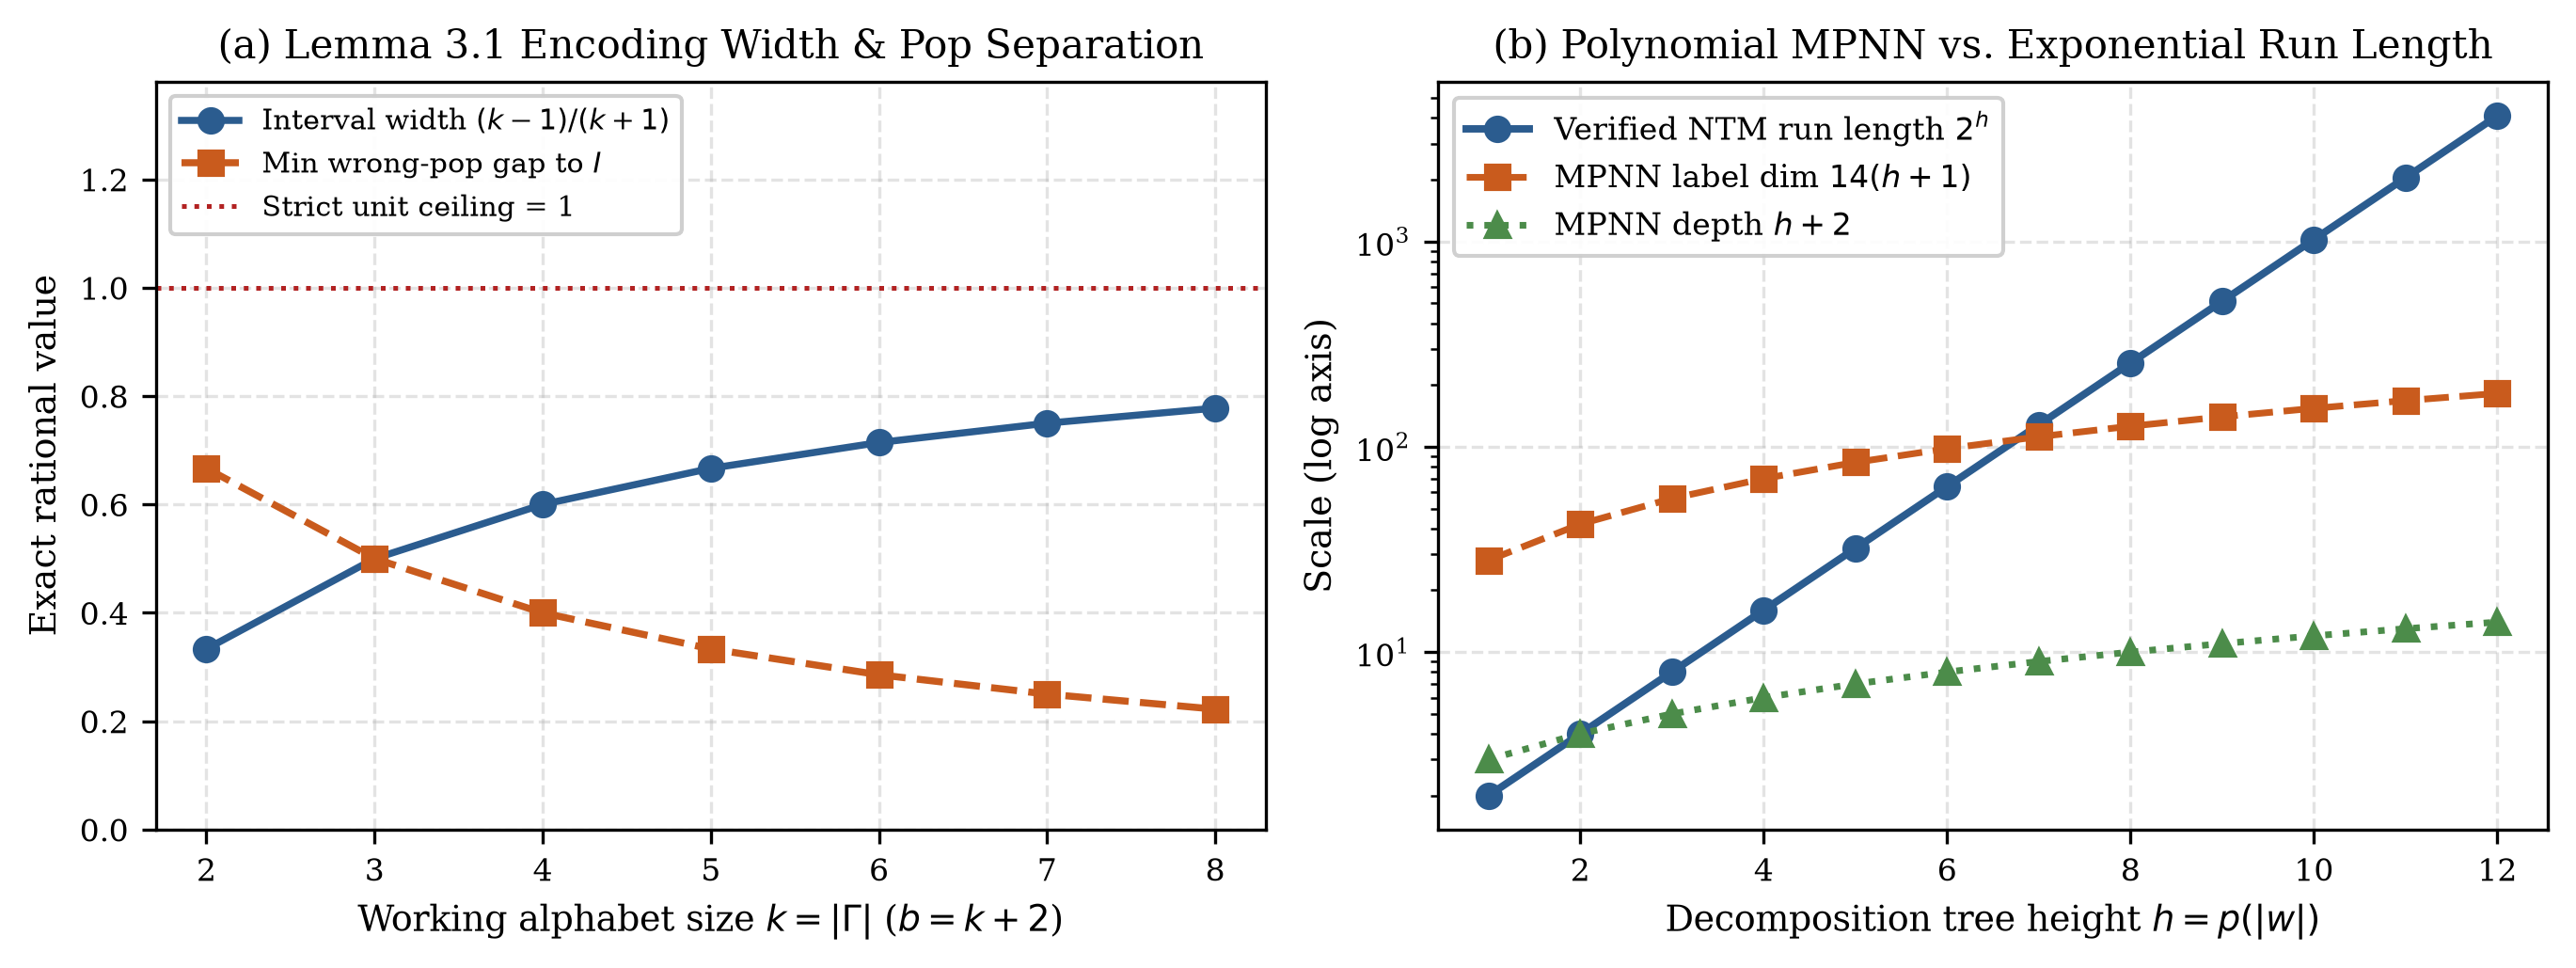
\includegraphics[width=\columnwidth]{../figures/fig1_encoding_and_scaling.png}
  \caption{(a) Lemma~3.1 interval width $(k-1)/(k+1) < 1$ and exact minimum wrong-pop distance to $I$ for $k = 2\dots 8$. (b) Exponential verified NTM run length $2^h$ vs.\ polynomial MPNN label dimension $14(h+1)$ and depth $h + 2$ ($h = 1\dots 12$).}
  \label{fig:enc}
\end{figure}

\paragraph{Encoding Separation and Polyhedral NTM Runs (Fig.~\ref{fig:enc}).}
Mode~1 ($0.080$--$0.093\,\mathrm{ms}$) verifies empty-tape fixed point $\enc(\epsilon) = 3/4$ ($k=3, b=5$) and multi-symbol words across $k \in \{3, 4, 6\}$ ($147/500$, $1777/3240$, $153299/229376$), confirming exact single-symbol $\pop$ disambiguation. Mode~2 ($5.394$--$20.855\,\mathrm{ms}$) audits 2-, 4-, and 8-step NTM runs (with both right/left head motion and accepting padding) across $|\Delta| \in \{18, 24\}$ six-dimensional rational polyhedra.

\begin{figure}[t]
  \centering
  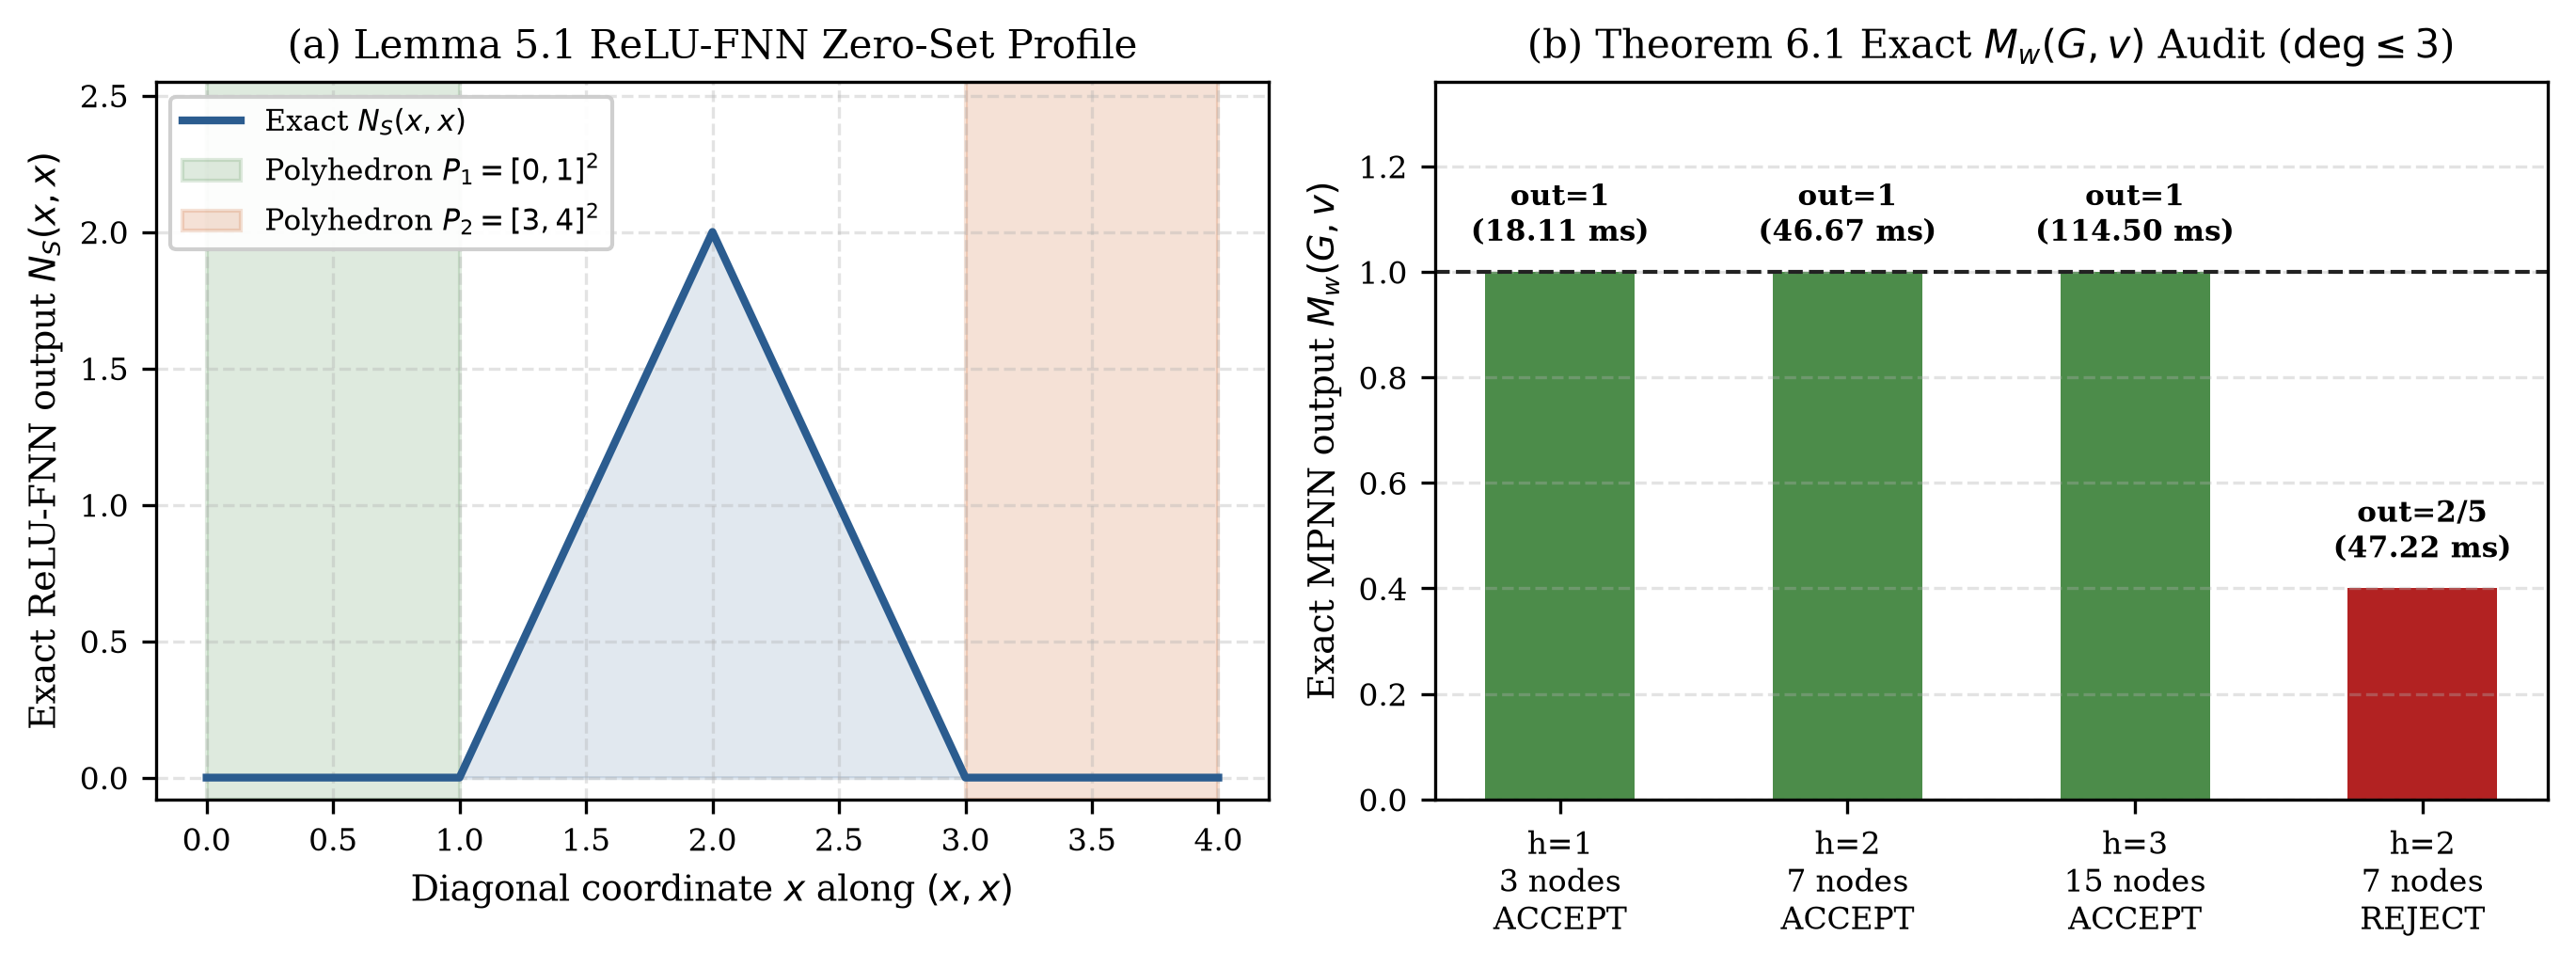
\includegraphics[width=\columnwidth]{../figures/fig2_relu_profile_and_mpnn_audit.png}
  \caption{(a) Exact Lemma~5.1 ReLU-FNN zero-set profile $N_S(x, x)$ along the diagonal across disjoint boxes $P_1 = [0,1]^2$ and $P_2 = [3,4]^2$ (zero iff $(x,x) \in S$, peaking at $2$ at $x=2$). (b) Mode~4 exact $(h+2)$-layer $M_w(G, v)$ outputs on degree-$\le 3$ witnesses: $1$ on $h=1,2,3$ accepting trees vs.\ $2/5$ (reject) on a corrupted leaf.}
  \label{fig:relu}
\end{figure}

\paragraph{ReLU-FNN Zero Sets and Full Degree-3 MPNN Execution (Fig.~\ref{fig:relu}).}
Mode~3 ($0.361$--$5.677\,\mathrm{ms}$) audits exact ReLU-FNN recognizers on 2D disjoint boxes, 3D non-convex unions, and actual NTM polyhedra $\mathcal{F} \subset \QQ^3$ and $\Delta \subset \QQ^6$. Mode~4 ($18.112$--$114.497\,\mathrm{ms}$) executes S\"alzer's exact $(h+2)$-layer MPNN $M_w$ on degree-$\le 3$ binary decomposition trees of heights $h=1$ ($3$ nodes, $28$-dim), $h=2$ ($7$ nodes, $42$-dim), and $h=3$ ($15$ nodes, $56$-dim, verifying an 8-step padded NTM run with $M_w(G,v)=1$), plus a soundness witness where perturbing one leaf coordinate by $+1/5$ propagates error $3/5$ to the root and yields exact rejection $M_w(G, v) = 2/5 \ne 1$.

\begin{figure}[t]
  \centering
  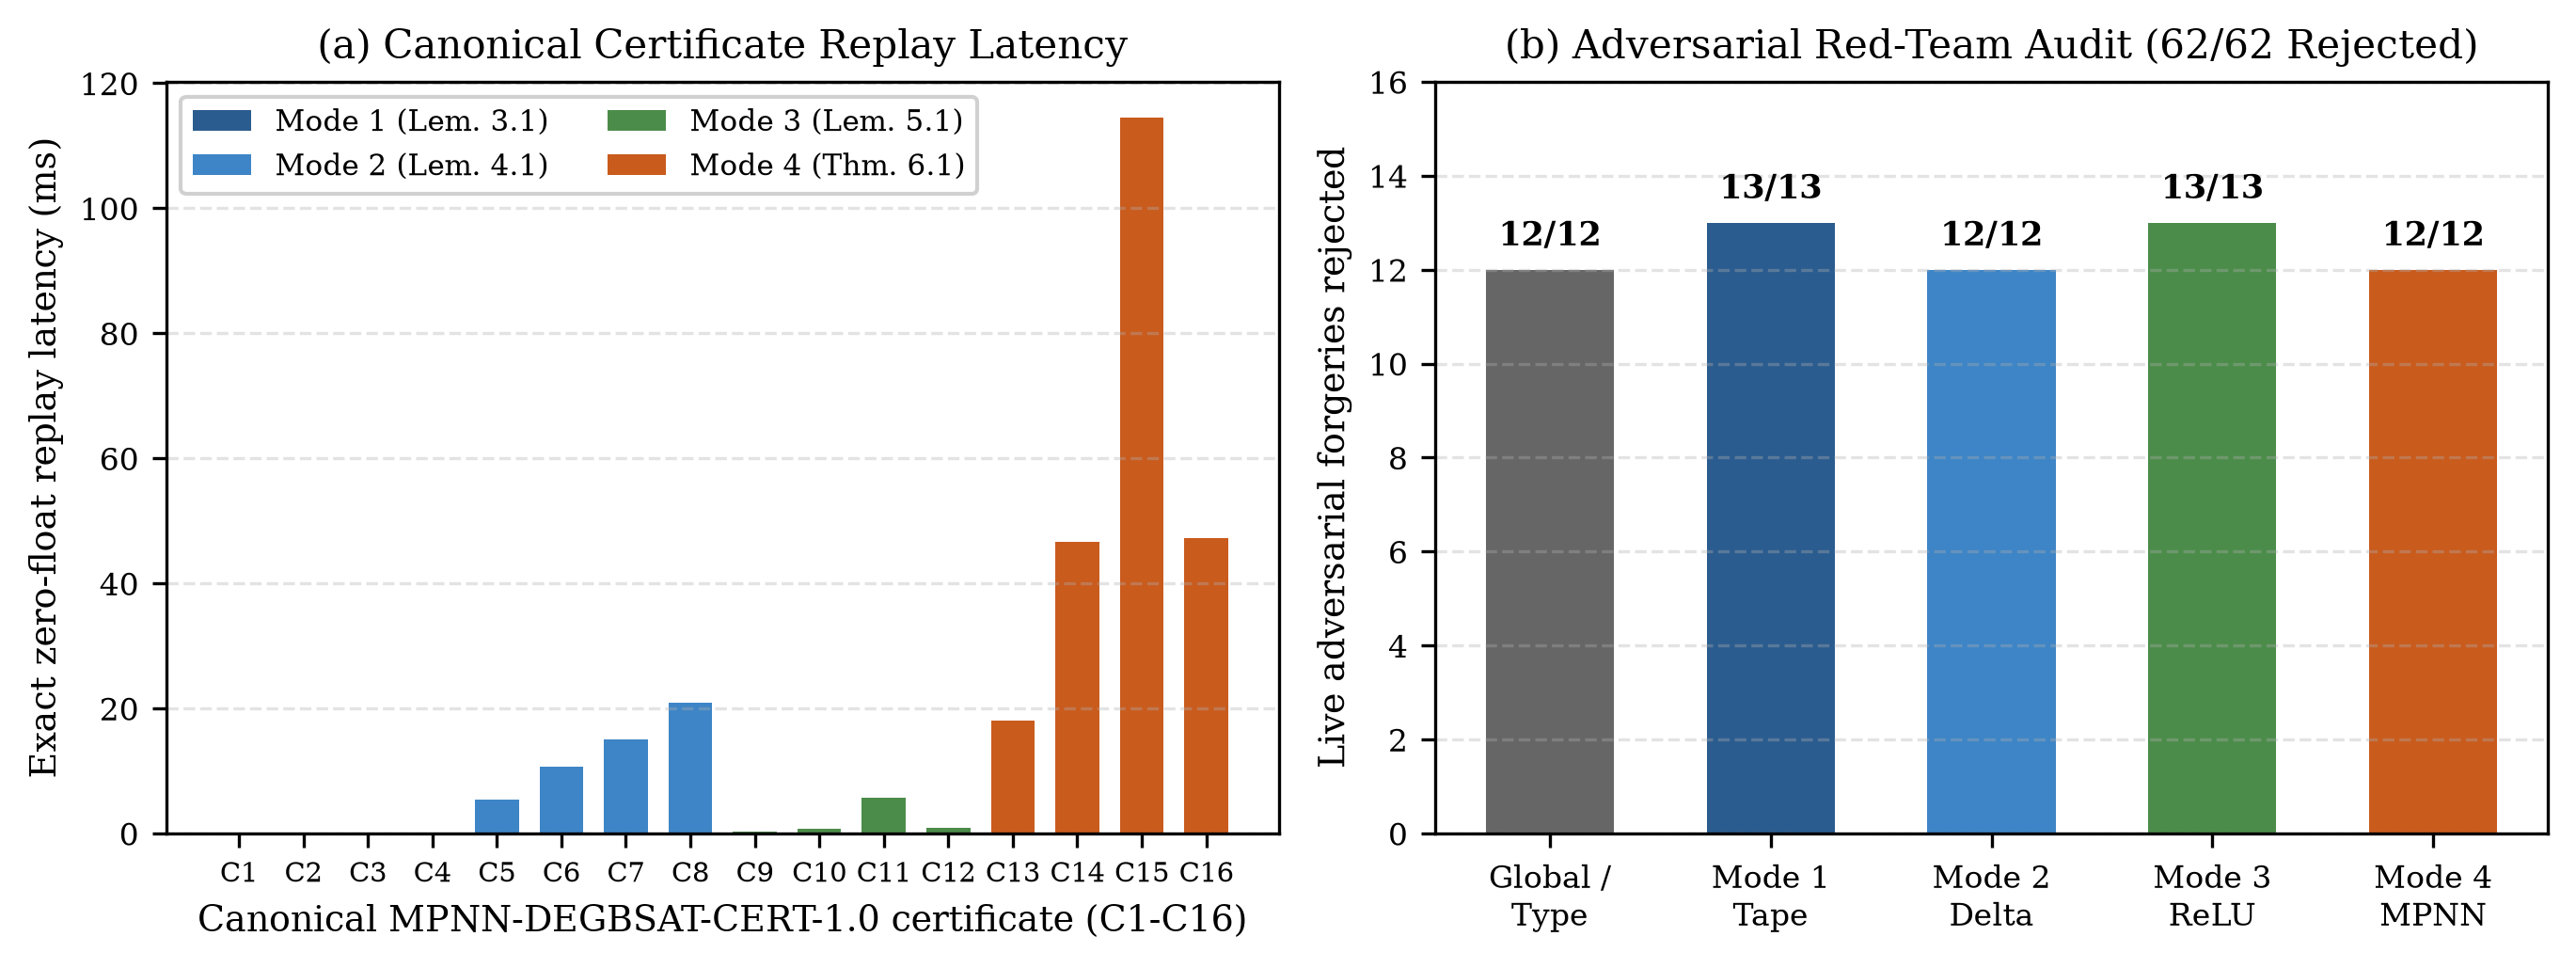
\includegraphics[width=\columnwidth]{../figures/fig3_certificate_replay_atlas.png}
  \caption{(a) Exact zero-float replay latency ($0.080$--$114.497\,\mathrm{ms}$) across all 16 canonical \texttt{MPNN-DEGBSAT-CERT-1.0} certificates. (b) Live adversarial red-team audit rejecting 62/62 forged payloads across all five categories.}
  \label{fig:atlas}
\end{figure}

\paragraph{Replay Latency and 62/62 Red-Team Audit (Fig.~\ref{fig:atlas}).}
All 16 canonical certificates replay in $0.080$--$114.497\,\mathrm{ms}$ (total $286.40\,\mathrm{ms}$). The live adversarial suite (\texttt{tests/test\_suite.py}) executes 62 targeted forgery attacks---12 global schema/type/rational/newline attacks plus 12--13 domain attacks per mode (invalid symbols, wrong pop flags, integer-as-boolean list confusion, duplicate/illegal NTM steps, non-accepting final states, trivial inside-only/outside-only Mode~3 queries, degree-$4$ graph violations, self-loops, wrong label dimensions, and forged acceptance on corrupted labels)---achieving \textbf{62/62 (100\%)} rejection.

\section{Conclusion}\label{sec:conc}
We delivered a self-contained, zero-floating-point verification stack for S\"alzer's $\NEXP$-hardness proof of fixed-degree ($d=3$) local-sum MPNN satisfiability~\cite{saelzer2026degbsat}, combining 18 zero-\texttt{sorry}, zero-\texttt{Classical.choice} Lean~4.35.0 theorems with the exact-$\QQ$ verifier \texttt{MPNN-DEGBSAT-CERT-1.0}, 16 canonical certificates (including full $(h+2)$-layer exact $M_w$ execution), and 62/62 adversarial forgery rejections.

\bibliographystyle{plain}
\bibliography{references}
\end{document}
